%%%%%%%%%%%%%%%%%%%%%%%%%%%%%%%%%%%%%%%%%%%%%%
%% Compile: XeLaTeX BibTeX XeLaTeX XeLaTeX
%% Loesung-Handout: Antonio Machicao y Priemer
%% Course: GK Linguistik
%%%%%%%%%%%%%%%%%%%%%%%%%%%%%%%%%%%%%%%%%%%%%%

%\documentclass[a4paper,10pt, bibtotoc]{beamer}
\documentclass[10pt,handout]{beamer}

%%%%%%%%%%%%%%%%%%%%%%%%
%%     PACKAGES      
%%%%%%%%%%%%%%%%%%%%%%%%

%%%%%%%%%%%%%%%%%%%%%%%%
%%     PACKAGES       %%
%%%%%%%%%%%%%%%%%%%%%%%%



%\usepackage[utf8]{inputenc}
%\usepackage[vietnamese, english,ngerman]{babel}   % seems incompatible with german.sty
%\usepackage[T3,T1]{fontenc} breaks xelatex
\usepackage{lmodern}

\usepackage{amsmath}
\usepackage{amsfonts}
\usepackage{amssymb}
%% MnSymbol: Mathematische Klammern und Symbole (Inkompatibel mit ams-Packages!)
%% Bedeutungs- und Graphemklammern: $\lsem$ Tisch $\rsem$ $\langle TEXT \rangle$ $\llangle$ TEXT $\rrangle$ 
\usepackage{MnSymbol}
%% ulem: Strike out
\usepackage[normalem]{ulem}  

%% Special Spaces (s. Commands)
\usepackage{xspace}				
\usepackage{setspace}
%	\onehalfspacing

%% mdwlist: Special lists
\usepackage{mdwlist}	

\usepackage[noenc,safe]{tipa}

% maybe define \textipa to use \originalTeX to avoid problems with `"'.
%
%	\ex \textipa{\originalTeX [pa.pa."g\t{aI}]}

%

\usepackage{etex}		%For Forest bug

%
%\usepackage{jambox}
%


%\usepackage{forest-v105}
%\usepackage{modified-langsci-forest-setup}

\usepackage{xeCJK}
\setCJKmainfont{SimSun}


%\usepackage{natbib}
%\setcitestyle{notesep={:~}}




% for toggles
\usepackage{etex}



% Fraktur!
\usepackage{yfonts}

\usepackage{url}

% für UDOP
\usepackage{adjustbox}


%% huberlin: Style sheet
%\usepackage{huberlin}
\usepackage{hu-beamer-includes-pdflatex}
\huberlinlogon{0.86cm}


%% Last Packages
%\usepackage{hyperref}	%URLs
%\usepackage{gb4e}		%Linguistic examples

% sorry this was incompatible with gb4e and had to go.
%\usepackage{linguex-cgloss}	%Linguistic examples (patched version that works with jambox

\usepackage{multirow}  %Mehrere Zeilen in einer Tabelle
%\usepackage{array}
\usepackage{marginnote}	%Notizen




%%%%%%%%%%%%%%%%%%%%%%%%%%%%%%%%%%%%%%%%%%%%%%%%%%%%
%%%          Commands                            %%%
%%%%%%%%%%%%%%%%%%%%%%%%%%%%%%%%%%%%%%%%%%%%%%%%%%%%

%%%%%%%%%%%%%%%%%%%%%%%%%%%%%%%%
% German quotation marks:
\newcommand{\gqq}[1]{\glqq{}#1\grqq{}}		%double
\newcommand{\gq}[1]{\glq{}#1\grq{}}			%simple


%%%%%%%%%%%%%%%%%%%%%%%%%%%%%%%%
% Abbreviations in German
% package needed: xspace
% Short space in German abbreviations: \,	
\newcommand{\idR}{\mbox{i.\,d.\,R.}\xspace}
\newcommand{\su}{\mbox{s.\,u.}\xspace}
%\newcommand{\ua}{\mbox{u.\,a.}\xspace}       % in abbrev
%\newcommand{\zB}{\mbox{z.\,B.}\xspace}       % in abbrev
%\newcommand{\s}{s.~}
%not possibel: \dh --> d.\,h.


%%%%%%%%%%%%%%%%%%%%%%%%%%%%%%%%
%Abbreviations in English
\newcommand{\ao}{a.o.\ }	% among others
\newcommand{\cf}[1]{(cf.~#1)}	% confer = compare
\renewcommand{\ia}{i.a.}	% inter alia = among others
\newcommand{\ie}{i.e.~}	% id est = that is
\newcommand{\fe}{e.g.~}	% exempli gratia = for example
%not possible: \eg --> e.g.~
\newcommand{\vs}{vs.\ }	% versus
\newcommand{\wrt}{w.r.t.\ }	% with respect to


%%%%%%%%%%%%%%%%%%%%%%%%%%%%%%%%
% Dash:
\newcommand{\gs}[1]{--\,#1\,--}


%%%%%%%%%%%%%%%%%%%%%%%%%%%%%%%%
% Rightarrow with and without space
\def\ra{\ensuremath\rightarrow}			%without space
\def\ras{\ensuremath\rightarrow\ }		%with space


%%%%%%%%%%%%%%%%%%%%%%%%%%%%%%%%
%% X-bar notation

%% Notation with primes (not emphasized): \xbar{X}
\newcommand{\MyPxbar}[1]{#1$^{\prime}$}
\newcommand{\xxbar}[1]{#1$^{\prime\prime}$}
\newcommand{\xxxbar}[1]{#1$^{\prime\prime\prime}$}

%% Notation with primes (emphasized): \exbar{X}
\newcommand{\exbar}[1]{\emph{#1}$^{\prime}$}
\newcommand{\exxbar}[1]{\emph{#1}$^{\prime\prime}$}
\newcommand{\exxxbar}[1]{\emph{#1}$^{\prime\prime\prime}$}

% Notation with zero and max (not emphasized): \xbar{X}
\newcommand{\zerobar}[1]{#1$^{0}$}
\newcommand{\maxbar}[1]{#1$^{\textsc{max}}$}

% Notation with zero and max (emphasized): \xbar{X}
\newcommand{\ezerobar}[1]{\emph{#1}$^{0}$}
\newcommand{\emaxbar}[1]{\emph{#1}$^{\textsc{max}}$}

%% Notation with bars (already implemented in gb4e):
% \obar{X}, \ibar{X}, \iibar{X}, \mbar{X} %Problems with \mbar!
%
%% Without gb4e:
\newcommand{\overbar}[1]{\mkern 1.5mu\overline{\mkern-1.5mu#1\mkern-1.5mu}\mkern 1.5mu}
%
%% OR:
\newcommand{\MyPibar}[1]{$\overline{\textrm{#1}}$}
\newcommand{\MyPiibar}[1]{$\overline{\overline{\textrm{#1}}}$}
%% (emphasized):
\newcommand{\eibar}[1]{$\overline{#1}$}
\newcommand{\eiibar}[1]{\overline{$\overline{#1}}$}

%%%%%%%%%%%%%%%%%%%%%%%%%%%%%%%%
%% Subscript & Superscript: no italics
\newcommand{\MyPdown}[1]{$_{\textrm{#1}}$}
\newcommand{\MyPup}[1]{$^{\textrm{#1}}$}


%%%%%%%%%%%%%%%%%%%%%%%%%%%%%%%%
% Objekt language marking:
%\newcommand{\obj}[1]{\glqq{}#1\grqq{}}	%German double quotes
%\newcommand{\obj}[1]{``#1''}			%English double quotes
\newcommand{\MyPobj}[1]{\emph{#1}}		%Emphasising


%%%%%%%%%%%%%%%%%%%%%%%%%%%%%%%%
%% Semantic types (<e,t>), features, variables and graphemes in angled brackets 

%%% types and variables, in math mode: angled brackets + italics + no space
%\newcommand{\type}[1]{$<#1>$}

%%% OR more correctly: 
%%% types and variables, in math mode: chevrons! + italics + no space
\newcommand{\MyPtype}[1]{$\langle #1 \rangle$}

%%% features and graphemes, in math mode: chevrons! + italics + no space
\newcommand{\abe}[1]{$\langle #1 \rangle$}


%%% features and graphemes, in math mode: chevrons! + no italics + space
\newcommand{\ab}[1]{$\langle$#1$\rangle$}  %%same as \abu  
\newcommand{\abu}[1]{$\langle$#1$\rangle$} %%Umlaute

%%% Notizen
\renewcommand{\marginfont}{\singlespacing}
\renewcommand{\marginfont}{\footnotesize}
\renewcommand{\marginfont}{\color{black}}

\newcommand{\myp}[1]{%
	\marginnote{%
		\begin{spacing}{1}
			\vspace{-\baselineskip}%
			\color{red}\footnotesize#1
		\end{spacing}
	}
}
%%%%%%%%%%%%%%%%%%%%%%%%%%%%%%%%
%% Outputbox
\newcommand{\outputbox}[1]{\noindent\fbox{\parbox[t][][t]{0.98\linewidth}{#1}}\vspace{0.5em}}

%%%%%%%%%%%%%%%%%%%%%%%%%%%%%%%%
%% (Syntactic) Trees
% package needed: forest
%
%% Setting for simple trees
\forestset{
	MyP edges/.style={for tree={parent anchor=south, child anchor=north}}
}

%% this is taken from langsci-setup file
%% Setting for complex trees
%% \forestset{
%% 	sn edges/.style={for tree={parent anchor=south, child anchor=north,align=center}}, 
%% background tree/.style={for tree={text opacity=0.2,draw opacity=0.2,edge={draw opacity=0.2}}}
%% }

\newcommand\HideWd[1]{%
	\makebox[0pt]{#1}%
}


%%%%%%%%%%%%%%%%%%%%%%%%%%%%%%%%%%%%%%%%%%%%%%%%%%%%
%%%          Useful commands                     %%%
%%%%%%%%%%%%%%%%%%%%%%%%%%%%%%%%%%%%%%%%%%%%%%%%%%%%

%%%%%%%%%%%%%%%%%%%%%
%% FOR ITEMS:
%\begin{itemize}
%  \item<2-> from point 2
%  \item<3-> from point 3 
%  \item<4-> from point 4 
%\end{itemize}
%
% or: \onslide<2->
% or: \pause

%%%%%%%%%%%%%%%%%%%%%
%% VERTICAL SPACE:
% \vspace{.5cm}
% \vfill

%%%%%%%%%%%%%%%%%%%%%
% RED MARKING OF TEXT:
%\alert{bis spätestens Mittwoch, 18 Uhr}

%%%%%%%%%%%%%%%%%%%%%
%% RESCALE BIG TABLES:
%\scalebox{0.8}{
%For Big Tables
%}

%%%%%%%%%%%%%%%%%%%%%
%% BLOCKS:
%\begin{alertblock}{Title}
%Text
%\end{alertblock}
%
%\begin{block}{Title}
%Text
%\end{block}
%
%\begin{exampleblock}{Title}
%Text
%\end{exampleblock}


\newtoggle{uebung}
\newtoggle{loesung}
\newtoggle{toc}

% The toc is not needed on Handouts. Safe trees.
\mode<handout>{
\togglefalse{toc}
}

\newtoggle{hpsgvorlesung}\togglefalse{hpsgvorlesung}
\newtoggle{syntaxvorlesungen}\togglefalse{syntaxvorlesungen}

%\includecomment{psgbegriffe}
%\excludecomment{konstituentenprobleme}
%\includecomment{konstituentenprobleme-hinweis}

\newtoggle{konstituentenprobleme}\togglefalse{konstituentenprobleme}
\newtoggle{konstituentenprobleme-hinweis}\toggletrue{konstituentenprobleme-hinweis}

%\includecomment{einfsprachwiss-include}
%\excludecomment{einfsprachwiss-exclude}
\newtoggle{einfsprachwiss-include}\toggletrue{einfsprachwiss-include}
\newtoggle{einfsprachwiss-exclude}\togglefalse{einfsprachwiss-exclude}

\newtoggle{psgbegriffe}\toggletrue{psgbegriffe}

\newtoggle{gb-intro}\togglefalse{gb-intro}



%%%%%%%%%%%%%%%%%%%%%%%%%%%%%%%%%%%%%%%%%%%%%%%%%%%%
%%%             Preamble's End                   
%%%%%%%%%%%%%%%%%%%%%%%%%%%%%%%%%%%%%%%%%%%%%%%%%%%% 

\begin{document}
	
	
%%%% ue-loesung
%%%% true: Übung & Lösungen (slides) / false: nur Übung (handout)
%	\toggletrue{ue-loesung}

%%%% ha-loesung
%%%% true: Hausaufgabe & Lösungen (slides) / false: nur Hausaufgabe (handout)
%	\toggletrue{ha-loesung}

%%%% toc
%%%% true: TOC am Anfang von Slides / false: keine TOC am Anfang von Slides
\toggletrue{toc}

%%%% sectoc
%%%% true: TOC für Sections / false: keine TOC für Sections (StM handout)
%	\toggletrue{sectoc}

%%%% gliederung
%%%% true: Gliederung für Sections / false: keine Gliederung für Sections
%	\toggletrue{gliederung}


%%%%%%%%%%%%%%%%%%%%%%%%%%%%%%%%%%%%%%%%%%%%%%%%%%%%
%%%             Metadata                         
%%%%%%%%%%%%%%%%%%%%%%%%%%%%%%%%%%%%%%%%%%%%%%%%%%%%      

\title{Grundkurs Linguistik}

\subtitle{Lösungen -- Syntax VI}

\author[A. Machicao y Priemer]{
	{\small Antonio Machicao y Priemer}
	\\
	{\footnotesize \url{http://www.linguistik.hu-berlin.de/staff/amyp}}
	%	\\
	%	\href{mailto:mapriema@hu-berlin.de}{mapriema@hu-berlin.de}}
}

\institute{Institut für deutsche Sprache und Linguistik}


% bitte lassen, sonst kann man nicht sehen, von wann die PDF-Datei ist.
%\date{ }

%\publishers{\textbf{6. linguistischer Methodenworkshop \\ Humboldt-Universität zu Berlin}}

%\hyphenation{nobreak}


%%%%%%%%%%%%%%%%%%%%%%%%%%%%%%%%%%%%%%%%%%%%%%%%%%%%
%%%             Preamble's End                  
%%%%%%%%%%%%%%%%%%%%%%%%%%%%%%%%%%%%%%%%%%%%%%%%%%%%      


%%%%%%%%%%%%%%%%%%%%%%%%%      
\huberlintitlepage[22pt]
\iftoggle{toc}{
	\frame{
		\begin{multicols}{2}
			\frametitle{Inhaltsverzeichnis}
			\tableofcontents
			%[pausesections]
			\columnbreak
%			\textcolor{white}{
%				\ea \label{ex:05cHA2}
%					\ea \label{ex:05cHA2a}
%					\ex \label{ex:05cHA2b}
%					\ex \label{ex:05cHA2c}
%					\z
%				\ex \label{ex:05cHA3}
%					\ea \label{ex:05cHA3a}
%					\ex \label{ex:05cHA3b}
%					\ex \label{ex:05cHA3c}
%					\ex \label{ex:05cHA3d}
%					\ex \label{ex:05cHA3e}
%					\z
%				\ex \label{ex:05cHA5}
%					\ea \label{ex:05cHA5a}
%					\ex \label{ex:05cHA5b}
%					\z
%				\ex \label{ex:05cHA6}
%				\ex \label{ex:05cHA7}
%				\ex \label{ex:05cHA9}
%				\z
%			}
		\end{multicols}
	}
}


%%%%%%%%%%%%%%%%%%%%%%%%%%%%%%%%%%%
%%%%%%%%%%%%%%%%%%%%%%%%%%%%%%%%%%%
\section{Übungen}

%%%%%%%%%%%%%%%%%%%%%%%%%%%%%%%%%%%
%06f Syntax ue-loesung01
%%%%%%%%%%%%%%%%%%%%%%%%%%%%%%%%%

\begin{frame}
\frametitle{Übung -- Lösung}


\begin{minipage}[b]{0.29\textwidth}
	\centering
	\scalebox{0.55}{
		\begin{forest}
			MyP edges,
			[CP
			[DP$ _{k} $[Das Kind, roof]]
			[\MyPxbar{C} 
			[\zerobar{C}[küsst$ _{i} $]]
			[IP
			[\alertgreen{t$_{k}$}]
			[\MyPxbar{I}
			[VP [\MyPxbar{V}
			[DP[die Mama, roof]]
			[\zerobar{V}[t$ _{i} $]]
			]
			]
			[\zerobar{I}[t$ _{i} $]]
			]
			]
			]
			]
		\end{forest}
		}
\end{minipage}
%
%
\begin{minipage}[b]{0.31\textwidth}
	\centering
	\scalebox{0.55}{
		\begin{forest}
			MyP edges,
			[CP
			[DP$ _{k} $[Das Kind, roof]]
			[\MyPxbar{C} 
			[\zerobar{C}[küsst$ _{i} $]]
			[IP
			[DP[die Mama, roof]]
			[\MyPxbar{I}
			[VP [\MyPxbar{V}
			[\alertgreen{t$_{k}$}]
			[\zerobar{V}[t$ _{i} $]]
			]
			]
			[\zerobar{I}[t$ _{i} $]]
			]
			]
			]
			]
		\end{forest}
		}
\end{minipage}
%%
%%
\begin{minipage}[b]{.38\textwidth}


\begin{itemize*}
	\alertgreen{\item {\small \MyPobj{das Kind} und \MyPobj{die Mama} sind im Akkusativ und im Nominativ formgleich (Synkretismus).}}
	\alertgreen{\item {\small Im Dt. kann eine Phrase in die SpecCP-Position bewegt werden.}}
	\alertgreen{\item {\small Wegen des Synkretismus' ist nicht ersichtlich, ob \MyPobj{das Kind} sich aus der SpecIP- oder aus der Schwesterposition von V\MyPup{0} bewegt hat. }}
\end{itemize*}

\end{minipage}
\end{frame}

%%%%%%%%%%%%%%%%%%%%%%%%%%%%%%%%%%%
%06f Syntax ue-loesung02
%%%%%%%%%%%%%%%%%%%%%%%%%%%%%%%%%

\begin{frame}
\frametitle{Übung -- Lösung}

\begin{minipage}[b]{0.45\textwidth}
	\centering
	\scalebox{0.6}{
		\begin{forest}
			MyP edges,
			[CP
			[DP$_{k}$ [Ich,roof]]
			[\MyPxbar{C} [\zerobar{C} [habe$_{i}$]]
			[IP [t$_{k}$]
			[\MyPxbar{I}
			[VP	[AdVP [heute,roof]]
			[VP [PP	[im Auto,roof]]{\draw[->,red] (.south west)--++(-7em,0em)--++(0em,14em)
				node[anchor=east,align=center]{PP kann nicht \\ bewegt werden};}
			[\MyPxbar{V} [\zerobar{V} [geschlafen t$_{i}$]]]
			]
			]
			[\zerobar{I} [t$_{i}$]]
			]
			]
			]	
			]
		\end{forest}
	}
\end{minipage}  
%            
%         
\begin{minipage}[b]{0.45\textwidth}
{\small 
	Nur eine Phrase, d.\,h.\ entweder die DP \MyPobj{ich} oder die PP \MyPobj{im Auto}, kann die SpecCP-Position belegen. Da die DP und die PP zusammen nicht eine Phrase bilden, können nicht \textbf{beide} Phrasen in diese Position bewegt werden.
}
\end{minipage}  

\end{frame}
%%%%%%%%%%%%%%%%%%%%%%%%%%%%%%%%%%%
%06f Syntax ue-loesung03
%%%%%%%%%%%%%%%%%%%%%%%%%%%%%%%%%%%
	
\begin{frame}
\frametitle{Übung -- Lösung}


\begin{columns}

\begin{column}{.45\textwidth}
\begin{figure}
	\scalebox{.6}{\begin{forest} sm edges,
			[S
			[VP [V [Tea] ] ]
			[NP
			[P [with]]
			[Det [some]]
			[N [lemon]]
			]
			[PP
			[P [tastes]]
			[NP [Adj [really] ] [N [nice]] ]
			]
			]
	\end{forest}}
	%	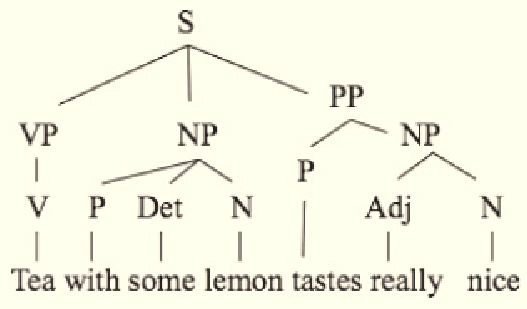
\includegraphics[scale=.45]{material/wrongtree}
	\caption{vgl.\ \url{http://specgram.com/CLXV.1/05.cruz-ferreira.know22.html}}
\end{figure}
\end{column}
%%
%%
\begin{column}{.55\textwidth}

\begin{itemize}
	\item keine binäre Struktur (mehr als zwei Töchter)
	\item falsche Kategorien bestimmt (\zB \MyPobj{Tea}: V?) 
	\item Es gibt Köpfe ohne Phrasen
	\item keine Zwischen Projektionen
	\item Satz ist exozentrisch
	\item \dots
\end{itemize}

\end{column}
\end{columns}

\end{frame}



%%%%%%%%%%%%%%%%%%%%%%%%%%%%%%%%%%%
%%%%%%%%%%%%%%%%%%%%%%%%%%%%%%%%%%%
\section{Hausaufgaben}

%%%%%%%%%%%%%%%
%06f Syntax ha-loesung
%%%%%%%%%%%%%%%%


\begin{frame}
\frametitle{Hausaufgabe -- Lösung}

\begin{itemize}
	\item Geben Sie an, um welchen \textbf{Phrasentyp} es sich bei den folgenden Phrasen handelt, und \textbf{welches Wort} sich in der \textbf{Kopfposition} der Phrasen befindet:
\end{itemize}	

\eal
	\ex viele besorgte Mütter  \pause \hfill \alertred{Mütter} \& \alertred{NP} oder \alertred{viele} \& \alertred{DP} \pause 

	\ex den Menschen in Not helfen \pause \hfill \alertred{helfen} \& \alertred{VP} \pause 
	
	\ex Wasser ohne Kohlensäure \pause \hfill \alertred{Wasser} \& \alertred{NP} oder \alertred{$\emptyset$} \& \alertred{DP} \pause 
	
	\ex auf Maria warten \pause \hfill \alertred{warten} \& \alertred{VP} \pause 
	
	\ex ob sie heute kommen werden \pause \hfill \alertred{ob} \& \alertred{CP} \pause 
	
	\ex Peter seine Traumfrau gefunden hat \pause \hfill \alertred{hat} \& \alertred{IP}
\zl

\end{frame}

%%%%%%%%%%%%%%%%%%%%%%%%%%%%%%%%%%%%%%

\begin{frame}
\frametitle{Hausaufgabe -- Lösung}

\begin{minipage}[b]{0.45\textwidth}
	
	{\small Peter schläft.}
	
	\pause
	
	\centering
	\scalebox{0.6}{
		\begin{forest}
			MyP edges,
			[CP 
			[DP$_{k}$ [Peter,roof]
			]
			[\MyPxbar{C}
			[\zerobar{C} [schläft$_{i}$]
			]
			[IP [t$_{k}$]
			[\MyPxbar{I}
			[VP [\MyPxbar{V} [\zerobar{V} [t$_{i}$	]]]]
			[\zerobar{I} [t$_{i}$]]
			]
			]
			]
			]
		\end{forest}
	}
\end{minipage}  
%            
%         
\begin{minipage}[b]{0.45\textwidth}
	
	\pause 
	
	{\small Wer schläft?}	
	
	\pause 
	
	\centering
	\scalebox{0.6}{
		\begin{forest}
			MyP edges,
			[CP 
			[DP$_{k}$ [Wer,roof]
			]
			[\MyPxbar{C}
			[\zerobar{C} [schläft$_{i}$]
			]
			[IP [t$_{k}$]
			[\MyPxbar{I}
			[VP [\MyPxbar{V} [\zerobar{V} [t$_{i}$	]]]]
			[\zerobar{I} [t$_{i}$]]
			]
			]
			]
			]
		\end{forest}
	}
\end{minipage}  

\end{frame}


%%%%%%%%%%%%%%%%%%%%%%%%%%%%%%%%%%
\begin{frame}
\frametitle{Hausaufgabe -- Lösung}

{\small Hat sie dir die schwierige Frage nach den Spuren gestellt?}

\pause

\begin{minipage}[b]{0.45\textwidth}

\centering
\scalebox{0.6}{
	\begin{forest}
		MyP edges,
		[CP 
		[\MyPxbar{C}
		[\zerobar{C} [Hat$_{i}$]
		]
		[IP [DP [\MyPxbar{D} [\zerobar{D} [sie]]]
		]
		[\MyPxbar{I}
		[VP 
		[DP [\MyPxbar{D} [\zerobar{D} [dir]]]]
		[\MyPxbar{V} 								
		[DP, draw, red 
		[die \dots\ Spuren,roof]
		]		
		[\zerobar{V} [gestellt]]
		]
		]
		[\zerobar{I} [t$_{i}$]]
		]
		]
		]
		]
	\end{forest}
}
\end{minipage}  
%      
\pause  	      
%         
\begin{minipage}[b]{0.45\textwidth}

\centering
\scalebox{0.4}{
	\begin{forest}
		MyP edges,
		[DP
		[\MyPxbar{D}
		[\zerobar{D}[die]]
		[NP
		[AP [\MyPxbar{A} [\zerobar{A} [schwierige]]]]
		[NP 
		[\MyPxbar{N} 
		[\zerobar{N} [Frage]]
		[PP
		[\MyPxbar{P} 
		[\zerobar{P} [nach]]
		[DP
		[\MyPxbar{D}
		[\zerobar{D} [den]]
		[NP [\MyPxbar{N} [\zerobar{N} [Spuren]]]]
		]
		]
		]
		]
		]
		]
		]
		]
		]
	\end{forest}
}
\end{minipage}  

\end{frame}


%%%%%%%%%%%%%%%%%%%%%%%%%%%%%%%%%%
\begin{frame}
\frametitle{Hausaufgabe -- Lösung}

{\small die fast vor dem Mittagessen erstellte Speisekarte}

\pause 

\begin{minipage}[b]{0.45\textwidth}

\centering
\scalebox{0.6}{
\begin{forest}
	MyP edges,
	[DP
	[\MyPxbar{D}
	[\zerobar{D}[die]]
	[NP
	[AP
	[PP, draw, red 
	[fast vor dem Mittagessen,roof]
	%							[AdvP [\MyPxbar{Adv} [\zerobar{Adv} [kurz]]]]
	%							[PP [\MyPxbar{P}
	%									[\zerobar{Adv} [vor]]
	%									[DP [\MyPxbar{D} [\zerobar{D} [dem]]
	%										[NP [\MyPxbar{N} [\zerobar{N} [Mittagessen]]]]
	%										]
	%									]				
	%								]							
	%							]
	]	
	[AP [\MyPxbar{A} [\zerobar{A} [erstellte]]]]
	]
	[NP [\MyPxbar{N} [\zerobar{N} [Speisekarte]]]
	]
	]
	]
	]
\end{forest}
}
\end{minipage}  
%  
\pause          
%         
\begin{minipage}[b]{0.45\textwidth}

\centering
\scalebox{0.6}{
\begin{forest}
	MyP edges,
	[PP 
	[AdvP [\MyPxbar{Adv} [\zerobar{Adv} [fast]]]]
	[PP 
	[\MyPxbar{P}
	[\zerobar{P} [vor]]
	[DP [\MyPxbar{D} [\zerobar{D} [dem]]
	[NP [\MyPxbar{N} [\zerobar{N} [Mittagessen]]]]
	]
	]				
	]							
	]
	]	
\end{forest}
}
\end{minipage}  

\end{frame}


%% -*- coding:utf-8 -*-

%%%%%%%%%%%%%%%%%%%%%%%%%%%%%%%%%%%%%%%%%%%%%%%%%%%%%%%%%


\def\insertsectionhead{\refname}
\def\insertsubsectionhead{}

\huberlinjustbarfootline


\ifpdf
\else
\ifxetex
\else
\let\url=\burl
\fi
\fi
\begin{multicols}{2}
{\tiny
%\beamertemplatearticlebibitems

\bibliography{gkbib,bib-abbr,biblio}
\bibliographystyle{unified}
}
\end{multicols}





%% \section{Literatur}
%% \begin{frame}[allowframebreaks]
%% \frametitle{Literatur}
%% 	\footnotesize

%% \bibliographystyle{unified}

%% 	%German
%% %	\bibliographystyle{deChicagoMyP}

%% %	%English
%% %	\bibliographystyle{chicago} 

%% 	\bibliography{gkbib,bib-abbr,biblio}
	
%% \end{frame}



\end{document}
